\clearpage
\pagenumbering{arabic}

\chapter{Introduction\label{Introduction}}


\section{Background\label{back}} 
The information and communications industry accounts for 3\% of the global electricity costs with an annual increase rate of 15 - 20\% \cite{green}. Base stations are responsible for more than half of the energy costs in the cellular network infrastructure \cite{residential}, indicating a huge demand to take advantage of renewable energy generation. Many countries have set green taxation and incentive schemes to achieve ambitious $CO_2$ emission reduction targets, making renewable energy harvesting technologies attractive for cellular network operators. Experts estimated that energy harvesting technology can reduce 20\% of the $CO_2$ emissions in the information and communications industry \cite{white_energy}.


Data traffic in cellular networks is growing rapidly \cite{7063493}. Recently, the traffic is growing 70 – 200\% per year \cite{wifi}.
As a result, base station (BS) densification is necessary for the implementation of 5G cellular networks and future generations of cellular networks \cite{SamarakoonSumudu2016UDSC}.
Dense deployment of BSs can meet the increasing traffic demand of new applications, such as ultra high definition video streaming, autonomous driving, and virtual reality based applications \cite{HetNets}. As a consequence, the accumulated BS energy consumption is rising considerably. To alleviate the impact on the environment and the cost burden on cellular network operators, photovoltaic (PV) cell powered BSs have been considered for future cellular networks \cite{residential, white_energy, Wang2015}. PV cells have been used for considerable time to power stand-alone BSs, which have no main grid connectivity \cite{NemaPragya2010Mogh}.
Compared with other renewable energy technologies, PV cells are often chosen to power a BS due to their small physical footprint in dense built environments, technology maturity, low maintenance cost, and production cost reduction in recent years \cite{white_energy}. 


Main grid energy is always on demand. In contrast, profiles of renewable energy harvesters have significant spatial \cite{Renewable_Power} and temporal variations \cite{HengWang2014Sqma}. In addition, the energy consumption profile of a BS is linked to the traffic load profile of the deployment area. For example, if the BS is located in a residential area, and in a business area, the energy consumption peak of the BS is at 23:00, and 11:30, respectively \cite{MarsanMarcoAjmone2013Tzge}. Consequently, the energy generation profile of a PV cell does not match the energy consumption profile of a BS in general \cite{TaoHan2014Pmnw}. The most common solutions to this problem reported in the literature are either energy storage technologies, such as batteries, supply side management, or demand side management \cite{LUTHANDER201580}.

This paragraph will highlight why demand side management is extremely difficult in a cellular network context. Demand side management at a BS is challenging, because it would imply to change the behavior of the users in terms of that they use their UEs at different times of the day or night. Users value cellular network services because of their convenience and always on demand property. A cellular network which is not always on demand would negatively affect the quality of service that the users expect from it. In more detail, that a BS needs less energy at a specific time of the day, fewer UEs have to request service, or less energy demanding jobs have to be requested by the UEs. This would mean in practice that users should use their UEs not during the day but rather at 3 am in the night or that users should not live screen ultra high definition videos but rather download videos in advance at 3 am in the night. Such a behavioral change is unlikely to happen due to the nature of the circadian rhythm of the human being. In addition, using a UE is often an impulse decision rather than a several hours in advanced planned decision.


Since demand side management is not an effective solution in a cellular network context, this thesis will focus on supply side management by deriving a new methodology based on orientation angle optimization to adjust the solar energy supply to meet the energy demand of the BS in the time domain. In addition, energy storage technologies, such as batteries, will also be evaluated in Chapter \ref{Chapter_2} in this thesis.



\section{PV Cell Angles\label{def_an}}
Section \ref{def_an} will define the two PV cell angels that are commonly used in the solar industry, which are denoted by orientation angle and inclination angle in this thesis. All angles in this thesis are in degrees.
Hence, all derived formulas, expressions, and statements in this thesis are given with respect to degrees and not radians. 


As shown in Figure \ref{angle}, the inclination angle of a PV cell, denoted by $\gamma$, is defined as the angle between the horizontal plane and the PV cell plane.
The orientation angle of a PV cell, denoted by $\theta$, is defined with respect to the southern direction.  Orientating the PV cell to the east (west) is indicated by a negative (positive) algebraic sign added to the orientation angle. For instance, the orientation angles of a PV cell orientated towards the east, south, and west are $\theta = - 90^{\mathrm{o}}$, $\theta = 0^{\mathrm{o}}$, and $\theta = 90^{\mathrm{o}}$, respectively.

\begin{figure}[H]
	\centering
		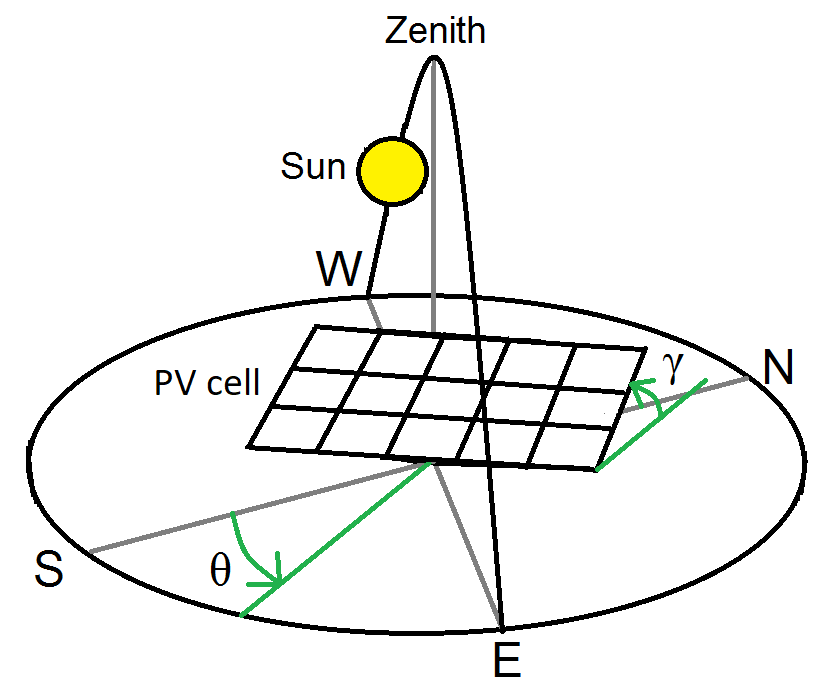
\includegraphics[width=0.6\textwidth]{pictures/nnnew}
\caption[Depiction of a PV cell installed with the orientation angle $\theta$ and inclination angle $\gamma$]{Depiction of a PV cell installed with the orientation angle $\theta=-30^{\mathrm{o}}$ and inclination angle $\gamma=20^{\mathrm{o}}$\label{angle}}
\end{figure}

The daily energy generation profile of a PV cell depends on the day of the year, the deployment location, the orientation angle $\theta$, and the inclination angle $\gamma$ of the PV cell.

The orientation and inclination angles of PV cells are usually fixed after the initial installation. Therefore, it is necessary to optimize the orientation and inclination angles of PV cells prior to the deployment. Without considering the energy consumption profile of the appliance, PV cells are deployed with default angles that are derived from the PV cell's geographic location as summarized in Table \ref{over}. The default inclination angle is set at a value similar to the latitude of the deployment area, and the default orientation angle is $0^{\mathrm{o}}$, and $180^{\mathrm{o}}$ in the northern, and southern hemispheres, respectively \cite{Solar_Cell}. Deploying PV cells with the default angles from Table \ref{over} guarantees that the PV cells harvest the most energy on a yearly timescale among all possible orientation and inclination angles. 





\begin{table}[H]
 \centering
\captionsetup{justification=centering}
\caption{\\ Default optimal orientation angle $\theta$ and inclination angle $\gamma$ for different locations \cite{Solar_Cell} \label{over}}
\label{overview}
\begin{tabularx}{\columnwidth}{@{}l*{2}{|C}Cc@{}}\toprule
\textbf{Location}					&  $\boldsymbol{\theta}$ 	&$\boldsymbol{\gamma}$ \\ \midrule
Northern hemisphere	& $0^{\mathrm{o}}$ 																&similar to the location's latitude						\\ 
Southern hemisphere	& $180^{\mathrm{o}}$ 															&similar to the location's latitude						\\ 
Equator							& any orientation angle &$0^{\mathrm{o}}$\\ \bottomrule
\end{tabularx}
\end{table}



This paragraph will investigate how the shape of the energy generation profile changes for different orientation angles on a daily timescale. 
Figure \ref{different_orientation_profiles} shows the daily energy generation profiles of southeast-oriented, south-oriented, and southwest-oriented PV cells, which are denoted by $G_{-45^{\mathrm{o}},1}(t)$, $G_{0^{\mathrm{o}},1}(t)$, and $G_{45^{\mathrm{o}},1}(t)$, respectively, for Greenwich (London, UK) during the summer. Orientating a PV cell eastwards (westwards) shifts the energy generation profile towards the morning (afternoon) hours in the northern hemisphere. The farther a PV cell is oriented away from the southern direction the less energy it harvests throughout the day. In other words, the more the energy generation profile peak is shifted away from noon the less energy is produced by the PV cell throughout the day. This tradeoff will be addressed in this thesis to determine the optimal orientation angle. 



\begin{figure}[H]
	\centering
		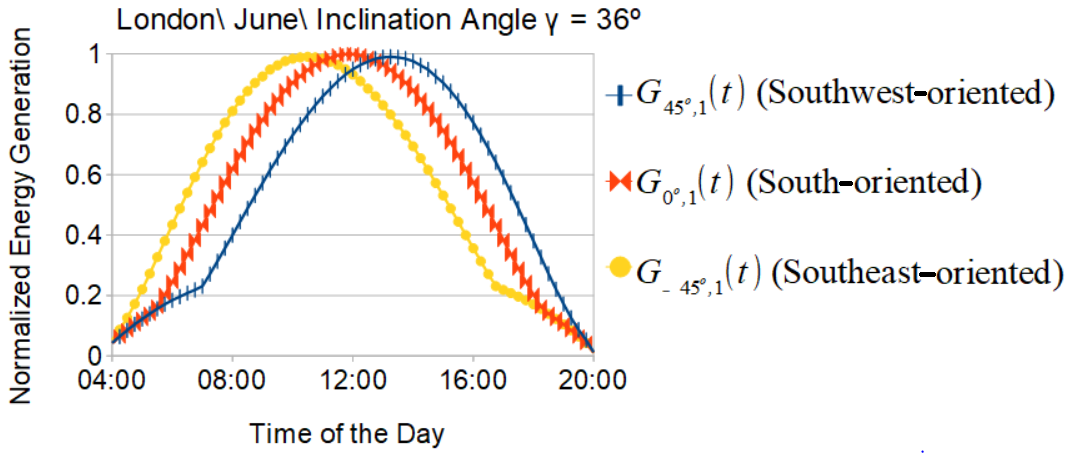
\includegraphics[width=1\columnwidth]{pictures/orien}
\caption{Effects of the orientation angle $\theta$ on the energy generation profile of the PV cell\label{different_orientation_profiles}}
\end{figure}

Optimizing the PV cell orientation angle is done on a daily timescale because it is a method to shift the energy generation peak from a surplus time (e.g. noon) to a deficit time (e.g. morning or afternoon), as seen in Figure \ref{different_orientation_profiles}. In contrast, optimizing the PV cell inclination angle is done on a yearly timescale because it is a method to shift the energy generation peak from a surplus season (e.g. summer) to a deficit season (e.g. winter). The focus of this thesis is to match the daily energy consumption profile of a BS with the daily energy generation profile of several PV cells. Hence, the orientation angles will be optimized in this thesis because the orientation angles affect the shape of the energy generation profile on a daily timescale. 




\section{Types of PV Cells\label{type_pv}}
PV cells can be classified into fixed, sun tracking, and adjustable PV cells (cf. \mbox{Figure \ref{ar}}). A fixed PV cell (cf. \mbox{Figure \ref{ar}(\subref{1})}) has fixed orientation and inclination angles which cannot be changed anymore after the initial installation. A single-axis sun tracking PV cell (cf. \mbox{Figure \ref{ar}(\subref{2})}) can mechanically track the sun throughout the day via adjusting the orientation angle. The single-axis sun tracking PV cell improves herein its daily energy yield compared with a fixed PV cell. A dual-axis sun tracking PV cell (cf. \mbox{Figure \ref{ar}(\subref{3})}) can mechanically track the sun throughout the day and the season, e.g., winter and summer, via adjusting both the orientation and inclination angles. The dual-axis sun tracking PV cell improves herein its yearly energy yield compared with a single-axis sun tracking PV cell. 


Despite the potentially higher energy yield of sun tracking PV cells than fixed PV cells, they are currently not widely deployed. The reasons are mainly the additional parts needed (e.g. axis motor), the higher maintenance (e.g. mechanical parts like the axis and the motor break more often than static parts), and the energy needed to operate the axis motor, which can be higher than the additional energy generated due to the sun tracking for some locations \cite{EKE20122665}. 


An adjustable PV cell (cf. \mbox{Figure \ref{ar}(\subref{4})}) requires an engineer to visit the site several times throughout the year to adjust the angles manually. Frequent (infrequent) adjustments of the angles will result in higher (lower) operational expenditure in combination with a higher (lower) energy yield of the PV cell. Due to the high wages in many countries, the increasing number of BSs in future cellular networks, and the problem that many BSs are difficult to access (e.g. on top of buildings or mountains), fixed PV cells are more suitable for powering BSs than adjustable PV cells. Hence, this thesis will focus on orientation angle optimization of fixed PV cells. Nonetheless, the derived optimization process in this thesis can equivalently be used to optimize the orientation angles of adjustable PV cells. For example, if the optimization method in this thesis is done on two days throughout the year (e.g. one day in winter, and one day in summer), the two derived optimal orientation angles can be altered every 6 months. The engineer should change the orientation angles of the adjustable PV cells during spring equinox and autumn equinox every year for this example. In general, fixed PV cells can be seen as a special case of an adjustable PV cell that does not require additional visits of engineers after its initial installation.





\begin{figure}[H]
\minipage{0.25\columnwidth}
  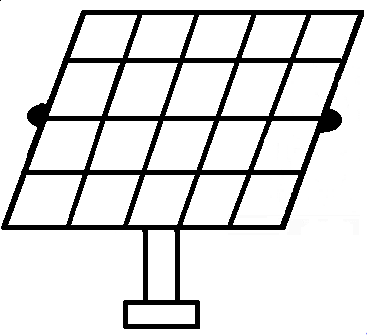
\includegraphics[width=\textwidth]{pictures/k1.png}
\subcaption{\label{1}}
\endminipage
\minipage{0.25\columnwidth}
  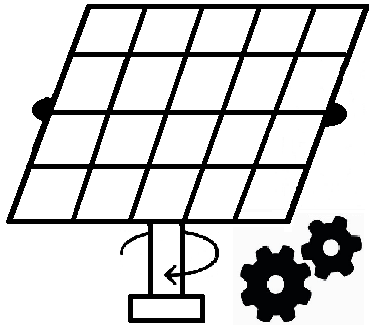
\includegraphics[width=\textwidth]{pictures/k2.png}
\subcaption{\label{2}}
\endminipage
\minipage{0.25\columnwidth}
  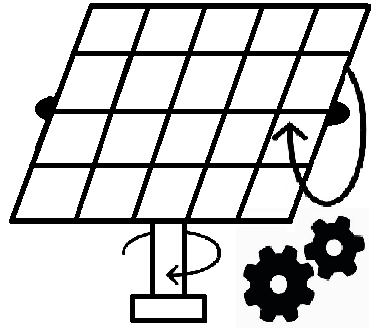
\includegraphics[width=\textwidth]{pictures/k3.png}
\subcaption{\label{3}}
\endminipage
\minipage{0.25\columnwidth}
  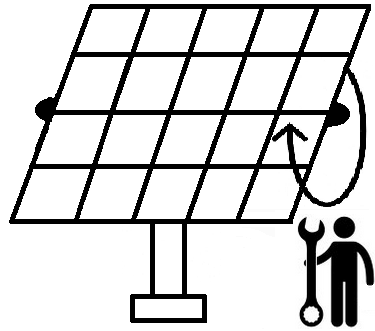
\includegraphics[width=\textwidth]{pictures/k5.png}
\subcaption{\label{4}}
\endminipage
\caption[Depiction of a fixed PV cell, a single-axis sun tracking PV cell, a dual-axis sun tracking PV cell, and an adjustable PV cell]{Depiction of a fixed PV cell (a), a single-axis sun tracking PV cell (b), a dual-axis sun tracking PV cell (c), and an adjustable PV cell (d) \label{ar}}
\end{figure}










